\subsection{Разработка имитатора пользовательских заявок}

\subsection*{Анализ исходного набора данных}
Исходные данные для построения статистической модели пользовательских
заявок представлены в виде набора учётных записей SLURM
\texttt{acct\_0921-0923}~\cite{schedmd2024sacct}, содержащего сведения о реально выполненных
задачах действующего вычислительного кластера. В соответствии с
вариантом задания из общего набора данных были отобраны записи,
удовлетворяющие условиям фильтрации: идентификатор пользователя \texttt{UID = 50430} и
имя задачи \texttt{JobName = "run\_bwa.sh"}.

В результате первичной фильтрации было получено $N_{\text{sample}} = 1433$
записи, послужившие основой для дальнейшего статистического анализа.

В ходе предварительного анализа отобранного подмножества выявлено
80~записей со статусом \texttt{COMPLETED} и фактическим временем
выполнения не более 10~секунд. Данные задачи относятся к одному
инфраструктурному событию 30~августа 2023~года и характеризуются аномально высоким
коэффициентом ошибки оценки~$\\\tau = T_{\text{заявки}} / T_{\text{факт}}$ в диапазоне от~7200 до~43200, что на два порядка
превышает типичные значения для нормальных задач ($\tau \approx 10$–$200$)~\cite{kappes2018userestimates,mualem2001utilization}.
Природа данной аномалии связана со сбоем вычислительного узла (\texttt{NODE\_FAIL})~\cite{di2014jobfailures}, после
которого планировщик зафиксировал аварийно завершенные и автоматически перезапущенные задачи как успешно
выполненные с околонулевым временем работы. Указанные записи были исключены
из расчёта параметров модели как артефакты инфраструктуры, не
характеризующие реальную пользовательскую нагрузку. Итоговая очищенная выборка
для статистического анализа составила \textbf{703~записи}.

\subsection*{Предварительный анализ и масштабирование данных}
Анализ распределения параметров показал, что фактическое время
выполнения пользовательских задач (\texttt{ElapsedRaw}) варьируется
в широком диапазоне от~$29$~секунд до~$10794$~секунд (около~3~часов).

\begin{figure}[H]
    \centering
    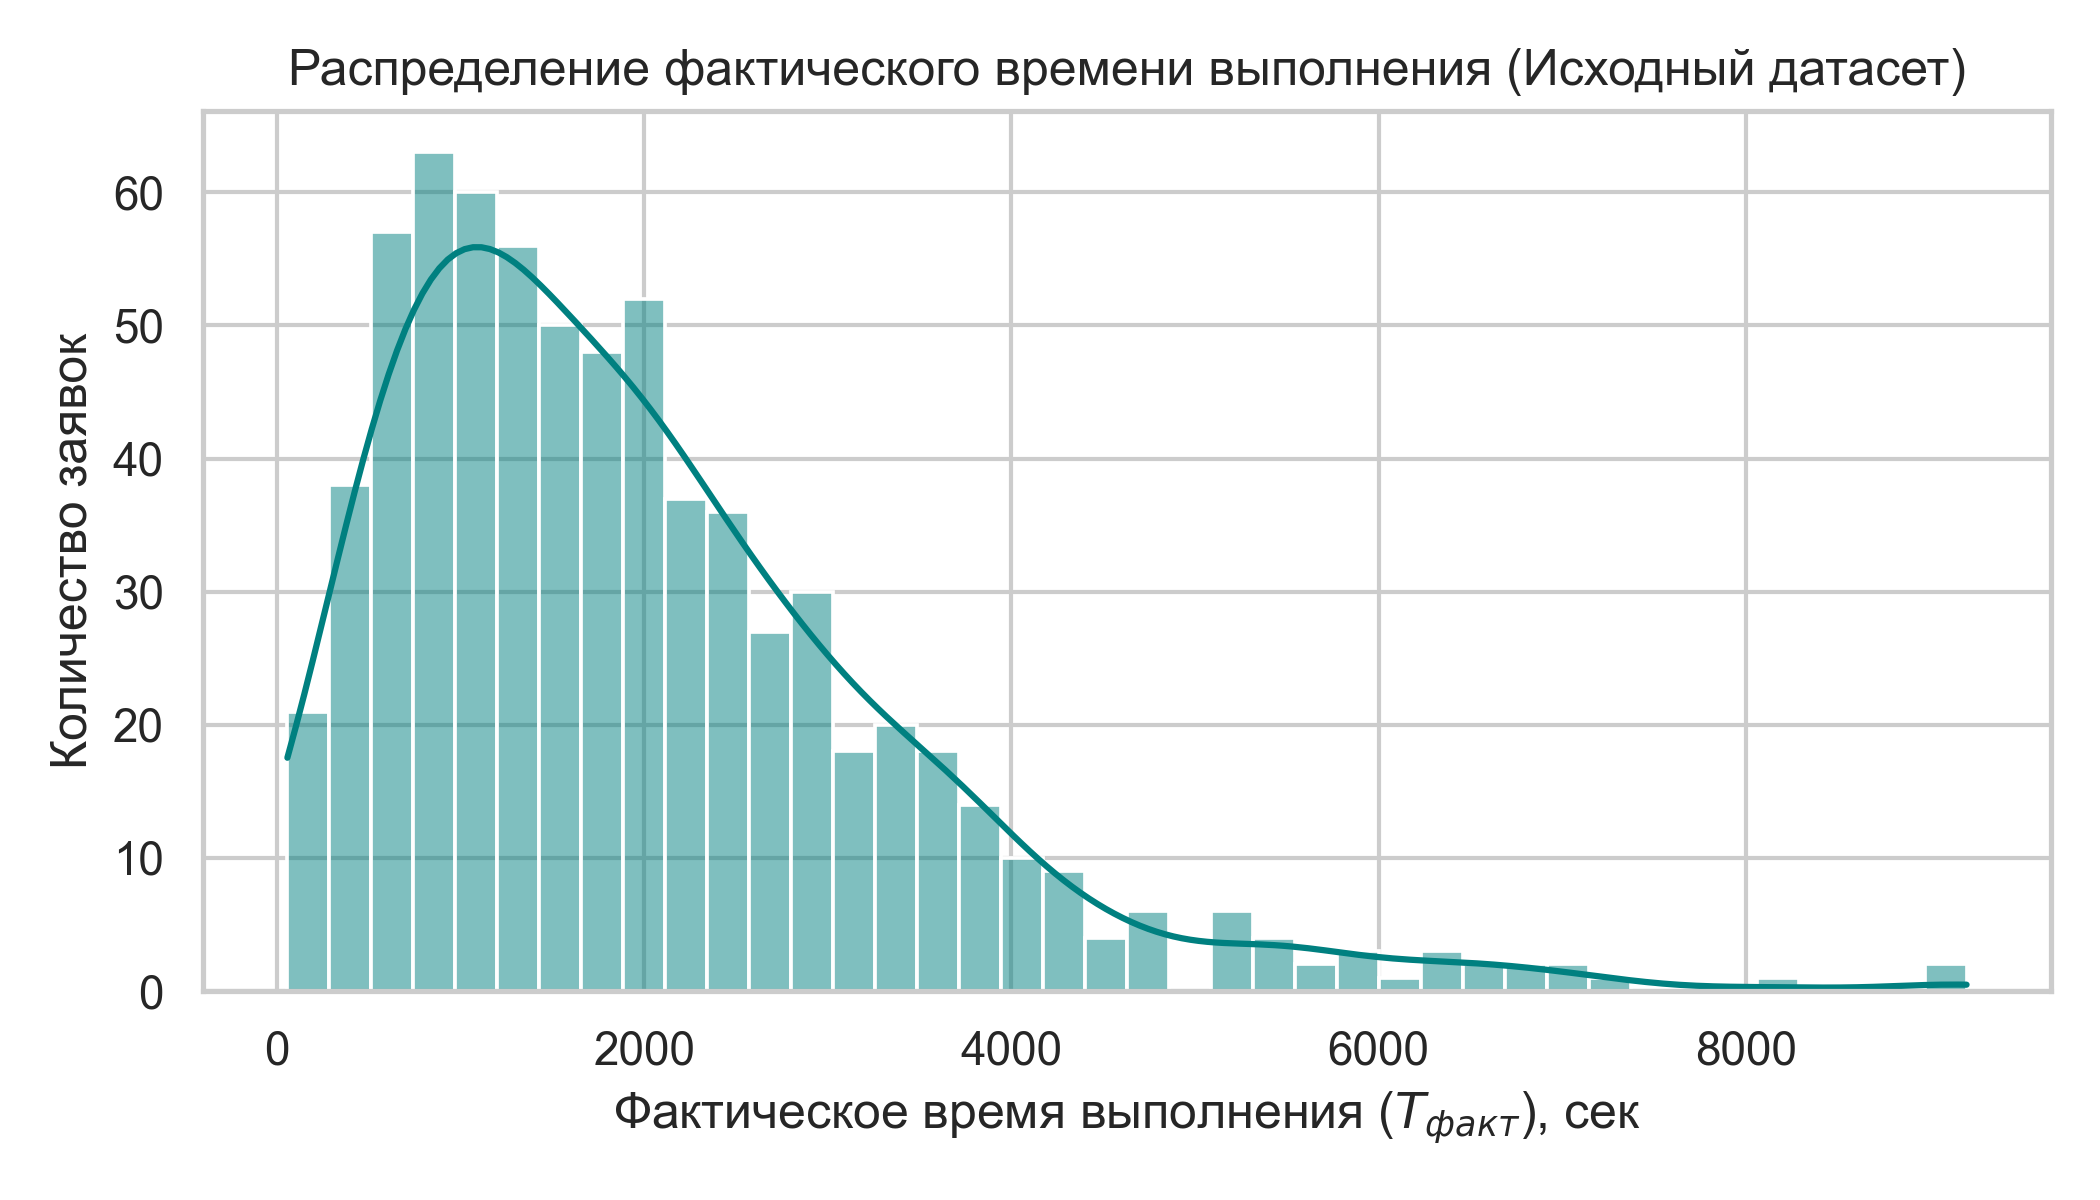
\includegraphics[width=0.85\textwidth]{figures/elapsed_distribution.png}
    \caption{Распределение фактического времени выполнения задач (исходный датасет acct\_0921-0923)}
    \label{fig:elapsed_distribution}
\end{figure}

Статистический анализ логарифмированных значений коэффициента
ошибки пользовательской оценки~($\ln\tau$) по~703~записям дал следующие
параметры распределения: математическое ожидание $\mu = 3{,}9411$ и среднеквадричное отклонение $\sigma = 0{,}8260$.
Данный график распределения подтверждает применимость логнормальной модели для описания ошибки пользовательской оценки времени выполнения задач данного типа~\cite{kappes2018userestimates,tsafrir2007backfilling}.

\begin{figure}[H]
    \centering
    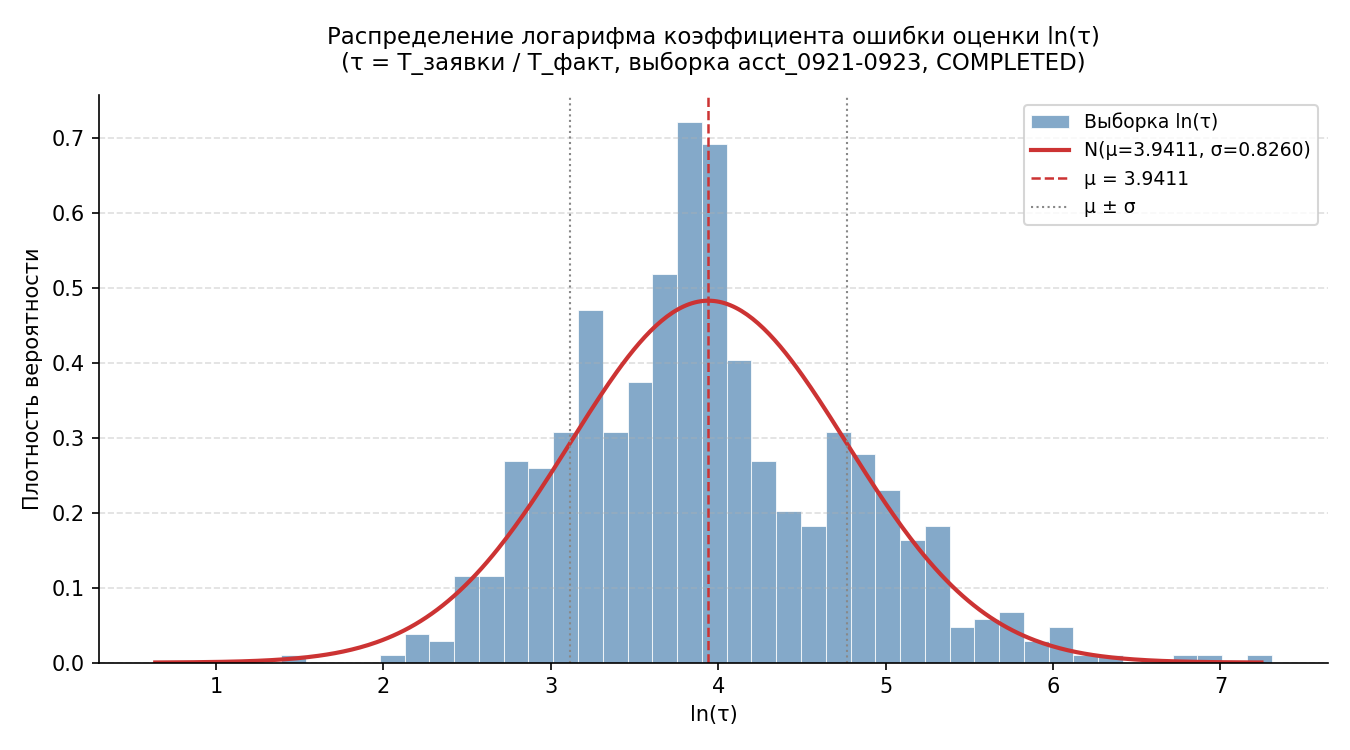
\includegraphics[width=0.85\textwidth]{figures/fig3_ln_tau_distribution.png}
    \caption{Распределение логарифма коэффициента ошибки оценки $\ln(\tau)$ на основе исторических данных}
    \label{fig:ln_tau_distribution}
\end{figure}

Широкий временной диапазон исходных задач существенно затрудняет их
непосредственное воспроизведение на учебном демонстрационном эксперименте. В связи с этим в процессе разработки было принято решение о временном масштабировании характеристик. Для финального тестирования и валидации модели выбран понижающий коэффициент масштабирования $k = 30$. Данное преобразование переводит диапазон выполнения основной массы заявок в интервалы от единиц секунд до единиц минут (максимальное масштабированное время составило 360 секунд, а медианное значение — около 30 секунд). Такой масштаб минимизирует интегральную ошибку округления диспетчера, сокращает общее время проведения эксперимента и сохраняет достаточную долю задач длительностью свыше одной минуты (${\approx}18\%$ выборки), что критически важно для корректного моделирования сценариев принудительного снятия задач планировщиком по таймауту.

Для снижения общей трудоемкости и ускорения валидации имитационной модели без потери статистической значимости, объем финальной тестовой выборки был установлен в размере примерно $0{,}5$ от величины исходного набора данных и составил $N_{\text{sim}} = 694$ заявки.

\subsection*{Выбор модели ошибки оценки времени выполнения}
Для количественной характеристики отклонения пользовательской оценки
времени выполнения от фактической длительности задачи использовались две альтернативные модели:
\begin{itemize}
\item абсолютное отклонение: $\Delta T = T_{\text{заявки}} - T_{\text{факт}}$;
\item относительный коэффициент ошибки: $\tau = T_{\text{заявки}} / T_{\text{факт}}$.
\end{itemize}

По результатам анализа было установлено, что дисперсия величины $\Delta T$ сильно зависит от масштаба самой задачи и часто превышает значение $T_{\text{факт}}$, в то время как относительный коэффициент $\tau$ инвариантен к длительности задачи. На основании этого для имитатора была выбрана логнормальная модель относительного отклонения~$\tau$~\cite{mualem2001utilization,tsafrir2007backfilling}.

\subsection*{Вычисление статистических параметров}
В таблице~\ref{tab:stats_comparison} приведены итоговые сопоставимые параметры исходного очищенного набора данных и результирующей масштабированной выборки, используемой в имитаторе.

\begin{table}[H]
\caption{Статистические параметры исходной и масштабированной выборок}
\label{tab:stats_comparison}
\centering
\begin{tabular}{|l|c|c|}
\hline
Параметр & Исходное значение & Масштабированное значение ($k=30$) \\
\hline
$T_{\text{факт, min}}$, с & 29     & 1   \\
$T_{\text{факт, max}}$, с & 10794  & 360 \\
$\mu$ ($\ln \tau$)        & 3,9411 & 3,9411 (не изменяется) \\
$\sigma$ ($\ln \tau$)     & 0,8260 & 0,8260 (не изменяется) \\
\hline
\end{tabular}
\end{table}

\subsection*{Алгоритм генерации пользовательской заявки}
Программная генерация параметров каждой синтетической заявки реализована на языке Python~\cite{python3docs} и состоит из трех последовательных шагов.

На \textbf{первом этапе} моделируется фактическое время выполнения задачи $T_{\text{факт}}$ как случайная величина, подчиненная нормальному закону распределения $\mathcal{N}(\mu_t, \sigma_t^2)$. Математическое ожидание и стандартное отклонение определяются на основе масштабированных границ исследуемой выборки:
\[
\mu_t = \frac{T_{\text{min}} + T_{\text{max}}}{2} = 180{,}5\text{ с}, \qquad
\sigma_t = \frac{T_{\text{max}} - T_{\text{min}}}{4} = 89{,}75\text{ с}.
\]
Данный выбор обеспечивает попадание более 95\% генерируемых значений в интервал $[T_{\text{min}},\, T_{\text{max}}]$. Ограничение диапазона сверху и снизу реализуется методом усечения (генерация в цикле до выполнения условия $1 \le T_{\text{факт}} \le 360$). В программном коде также предусмотрено жесткое ограничение:
\begin{equation}
T_{\text{факт}} = \max(2, \mathrm{round}(T_{\text{факт}}))
\end{equation}
Введение нижней граничной константы в $2$ секунды технически обосновано необходимостью исключить генерацию сверхкоротких задач ($1$ с), для которых накладные расходы на вызов системного таймера и инициализацию интерпретатора сопоставимы с временем работы самой задачи, что приводит к значительным погрешностям при округлении интервалов.

На \textbf{втором этапе} моделируется коэффициент пользовательской ошибки перестраховки $\tau \sim \mathrm{LogNormal}(\mu, \sigma^2)$ с параметрами $\mu = 3{,}9411$ и $\sigma = 0{,}8260$. Плановое запрашиваемое время вычисляется как:
\[
T_{\text{заявки}} = \mathrm{round}(T_{\text{факт}} \cdot \tau)
\]
Если сгенерированное значение удовлетворяет неравенству $T_{\text{заявки}} \le T_{\text{факт}}$, лимит времени принудительно корректируется добавлением случайной величины в диапазоне $[5, 15]$ секунд, что гарантирует штатное выполнение задачи.

На \textbf{третьем этапе} учитывается специфика работы пакетного диспетчера SLURM: директива лимита времени \texttt{--time} в формате \texttt{MM:SS} принудительно округляется планировщиком вверх до ближайшей целой минуты. Следовательно, при сильном масштабировании короткие задачи гарантированно успевают завершиться в рамках выделенного минутного кванта, из-за чего механизм принудительного снятия по таймауту (\texttt{TIMEOUT}) диспетчером зафиксирован не будет. Для обеспечения возможности полноценного тестирования и валидации подсистемы обработки прерываний, вероятность генерации таймаутных заявок искусственно увеличена в рамках эксперимента. Принудительный таймаут моделируется только для задач с $T_{\text{факт}} > 60$ с, при этом плановый лимит времени $T_{\text{заявки}}$ устанавливается строго краттным 60 секундам и гарантированно меньшим, чем реальное время выполнения задачи $T_{\text{факт}}$.

Количество запрашиваемых задачей вычислительных узлов моделируется как дискретная случайная величина, распределенная равномерно на множестве $\{1, 2, 3, 4\}$.

\subsection*{Реализация программы-имитатора и структура данных}
Программа-имитатор реализована в виде скрипта \texttt{simulator.py}. Перед запуском цикла генерации скрипт производит очистку целевого каталога \texttt{/home/vlad/saved\_jobs} и открывает на перезапись файлы логирования. В процессе работы формируются три типа файлов данных, структуры которых подробно описаны в таблицах \ref{tab:csv_plan}, \ref{tab:csv_fact} и \ref{tab:csv_overhead}.

\begin{table}[H]
\caption{Структура файла внутренней статистики \texttt{simulation\_stats.csv}}
\label{tab:csv_plan}
\centering
\small
\begin{tabular}{|l|l|p{7.5cm}|}
\hline
Поле & Тип & Описание \\
\hline
\texttt{Timestamp}          & строка  & Дата и время генерации параметров задачи (ГГГГ-ММ-ДД ЧЧ:ММ:СС) \\
\texttt{SimID}              & целое   & Внутренний порядковый номер заявки в имитаторе \\
\texttt{SlurmJobID}         & целое   & Идентификатор, присвоенный задаче планировщиком SLURM \\
\texttt{Nodes}              & целое   & Количество запрошенных вычислительных узлов ($1$–$4$) \\
\texttt{PlannedTime\_Sec}   & целое   & Сгенерированный плановый лимит времени $T_{\text{заявки}}$, с \\
\texttt{ActualTime\_Sec}    & целое   & Смоделированное базовое фактическое время выполнения $T_{\text{факт}}$, с \\
\texttt{Tau}                & вещест. & Реализованный коэффициент ошибки оценки $\tau = T_{\text{заявки}} / T_{\text{факт}}$ \\
\texttt{IsTimeout}          & бинарн. & Флаг отнесения заявки к категории таймаутных ($0$ — нет, $1$ — да) \\
\hline
\end{tabular}
\end{table}

\begin{table}[H]
\caption{Структура системного лога планировщика \texttt{slurm\_real\_fact.txt}}
\label{tab:csv_fact}
\centering
\small
\begin{tabular}{|l|l|p{8.5cm}|}
\hline
Поле & Тип & Описание \\
\hline
\texttt{JobID}      & целое  & Уникальный идентификатор задачи в подсистеме учета SLURM \\
\texttt{JobName}    & строка & Имя запущенного пакетного скрипта (\texttt{run\_bwa.sh}) \\
\texttt{Nodes}      & целое  & Фактически выделенное количество вычислительных узлов \\
\texttt{State}      & строка & Терминальный статус задачи (\texttt{COMPLETED}, \texttt{TIMEOUT}) \\
\texttt{ElapsedRaw} & целое  & Фактическое время выполнения задачи по часам SLURM, с \\
\hline
\end{tabular}
\end{table}

\begin{table}[H]
\caption{Структура лога высокоточного таймера \texttt{overhead\_log.csv}}
\label{tab:csv_overhead}
\centering
\small
\begin{tabular}{|l|l|p{8.5cm}|}
\hline
Поле & Тип & Описание \\
\hline
\texttt{SlurmJobID}           & целое & Идентификатор задача в планировщике \\
\texttt{SleepRequested\_Sec}  & целое & Длительность вычислительной нагрузки, переданная в команду \texttt{sleep}, с \\
\texttt{ActualElapsed\_Ms}    & целое & Полное время выполнения обертки задачи, измеренное утилитой \texttt{date} с точностью до миллисекунды, мс \\
\hline
\end{tabular}
\end{table}

Каждая сгенерированная задача экспортируется в текстовый файл сценария \texttt{sbatch}~\cite{schedmd2024sbatch}, содержащий директивы выделения ресурсов. Для проведения детального исследования накладных расходов диспетчеризации в тело каждого сценария встроен независимый замер времени аппаратными средствами ОС до и после выполнения полезной нагрузки с точностью до миллисекунды (с использованием системного вызова \texttt{date +\%s\%3N}):
\begin{verbatim}
START=$(date +%s%3N)
sleep <T_fact>
END=$(date +%s%3N)
\end{verbatim}
Разность этих меток фиксируется в файле \texttt{overhead\_log.csv}, что позволяет оценить системные задержки, которые SLURM не учитывает в своем стандартном логе, ведущемся дискретно до секунд.

Ниже приведены сопоставимые фрагменты полученных файлов данных для первых пяти задач симуляционного эксперимента.

\begin{lstlisting}[caption={Фрагмент файла внутренней статистики имитатора simulation\_stats.csv}]
Timestamp,SimID,SlurmJobID,Nodes,PlannedTime_Sec,ActualTime_Sec,Tau,IsTimeout
2026-06-29 15:46:43,1,1294,3,16208,316,51.2927,0
2026-06-29 15:46:50,2,1295,4,8355,254,32.8953,0
2026-06-29 15:47:02,3,1296,1,23453,305,76.8959,0
2026-06-29 15:47:16,4,1297,4,27753,208,133.4287,0
2026-06-29 15:47:24,5,1298,3,22791,246,92.6476,0
\end{lstlisting}

\begin{lstlisting}[caption={Фрагмент системного лога планировщика slurm\_real\_fact.txt}]
JobID|JobName|Nodes|State|ElapsedRaw
1294|run_bwa.sh|3|COMPLETED|316
1295|run_bwa.sh|4|COMPLETED|254
1296|run_bwa.sh|1|COMPLETED|305
1297|run_bwa.sh|4|COMPLETED|208
1298|run_bwa.sh|3|COMPLETED|246
\end{lstlisting}

\begin{lstlisting}[caption={Фрагмент лога накладных расходов overhead\_log.csv}]
SlurmJobID,SleepRequested_Sec,ActualElapsed_Ms
1294,316,316048
1295,254,254103
1296,305,305017
1297,208,208060
1298,246,246104
\end{lstlisting}

Сопоставление полей \texttt{ActualTime\_Sec} из лога имитатора и \texttt{ElapsedRaw} из лога планировщика наглядно подтверждает точность воспроизведения временных параметров в состоянии \texttt{COMPLETED}. Анализ данных файла \texttt{overhead\_log.csv} показывает наличие систематических накладных расходов диспетчеризации (величина задержки инициализации лежит в диапазоне от 17 до 104 мс), детальное исследование которых приведено в следующем аналитическом разделе работы.